\subsection{Analysis of observation statistics for Galileo}%
\label{subsec:AnalysisofobservationstatisticsforGalileo}%
\setlength{\tabcolsep}{4pt}%
\begin{longtabu}[c]{rcl}%
statistics observation file&:&SEPT00BEL\_R\_20203491400\_30M\_01S\_MO\_E.obsstat\\%
navigation signals&:&E1C\\%
\end{longtabu}%
\subsubsection{Observables count per navigation signal}%
\label{ssubsec:Observablescountpernavigationsignal}%
The following table represents the number of observations made for each examined navigation signal. The percentages per navigation signal are calculated by dividing by the  number of observations obtained from Two Line Elements (TLE) at the recorded interval. The last column represents the number of observations possible during the observed time interval.%
\setlength{\tabcolsep}{4pt}%
\begin{longtabu}[c]{l|rr|r}%
\textbf{PRN}&\textbf{E1C}&\textbf{}&\textbf{TLE\_count}\\%
\hline%
\endhead%
\hline%
\multicolumn{4}{r}{Continued on Next Page}\\%
\hline%
\endfoot%
\hline%
\endlastfoot%
E02&1503&83.5\%&1800.0\\%
E03&1524&84.7\%&1800.0\\%
E05&1491&82.8\%&1800.0\\%
E07&29&4.3\%&670.0\\%
E08&1524&84.7\%&1800.0\\%
E24&1492&82.9\%&1800.0\\%
E25&1521&84.5\%&1800.0\\%
E26&625&34.7\%&1800.0\\%
E33&118&6.6\%&1800.0\\%
\end{longtabu}%
Figure \ref{fig:obst_gnss_E} represents the absolute count of observables for each navigation signal set out against the maximum possible observations obtained from the TLEs. The relative observation count is represented in Figure \ref{fig:prec_obst_gnss_E}.%


\begin{figure}[H]%
\centering%
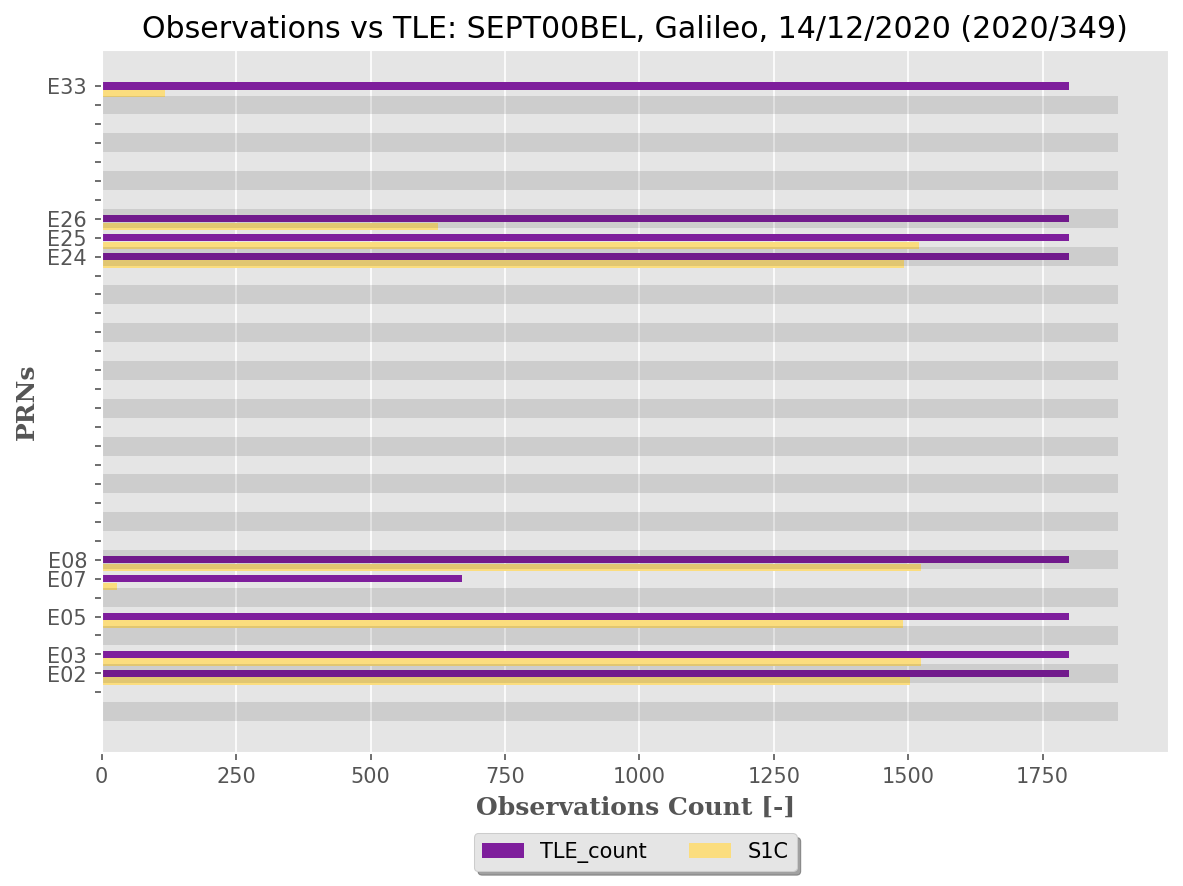
\includegraphics[width=0.95\textwidth]{png/SEPT00BEL_R_20203491400_30M_01S_MO_E-ObsTLE.png}%
\caption{\label{fig:obst_gnss_E} Observables overview for GNSS Galileo}%
\end{figure}

%


\begin{figure}[H]%
\centering%
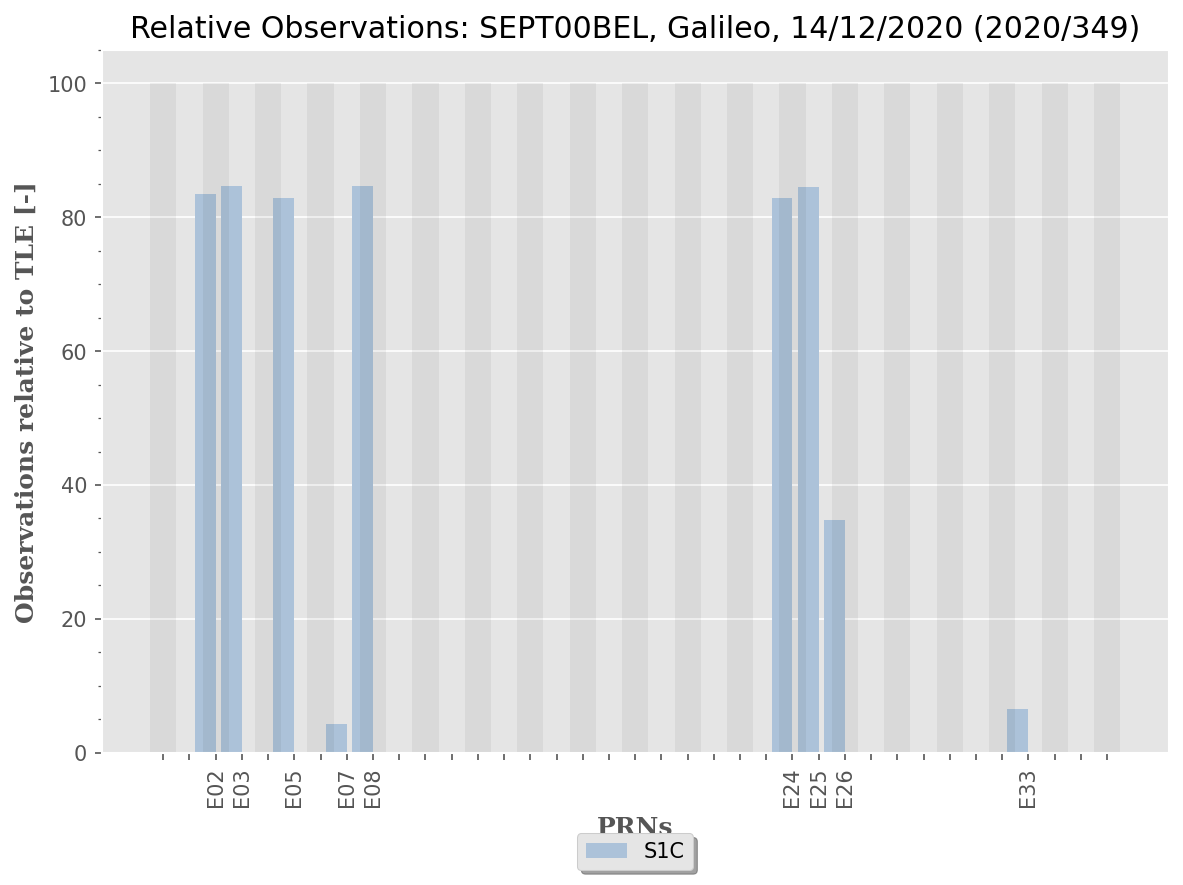
\includegraphics[width=0.95\textwidth]{png/SEPT00BEL_R_20203491400_30M_01S_MO_E-PERC.png}%
\caption{\label{fig:prec_obst_gnss_E} Relative observation count per navigation signal for GNSS Galileo}%
\end{figure}

%
\clearpage

